\subsection{Como o Flux funciona?}

Esta seção irá esclarecer como o Flux denomina cada parte do BPM e como é feita sua criação para implementação dentro do mesmo. Essas definições serão importantes para melhor leitura das implementações feitas no Flux para resolverem os problemas falados.

\subsubsection{Atributos, Atividades e Instâncias}

Os atributos de uma atividade definem as informações que poderão ser acrescentadas a uma atividade, isto é, os atributos definem quais dados poderão ser adicionados a cada atividade, definindo também seu tipo (número, texto...), obrigatoriedade, correlação com outros atributos, e um conjunto de atributos em um passo específico de um workflow forma uma atividade.

Uma atividade em um workflow define um passo no BPM modelado. Em um workflow, podem existir qualquer número de atividades, sendo uma atividade inicial para iniciar o BPM, seguido de atividades dependentes das atividades anteriores em um formato de árvore na definição computacional, como podemos ver na figura \ref{fig:bpmn_diagram}

\begin{figure}
    \centering
    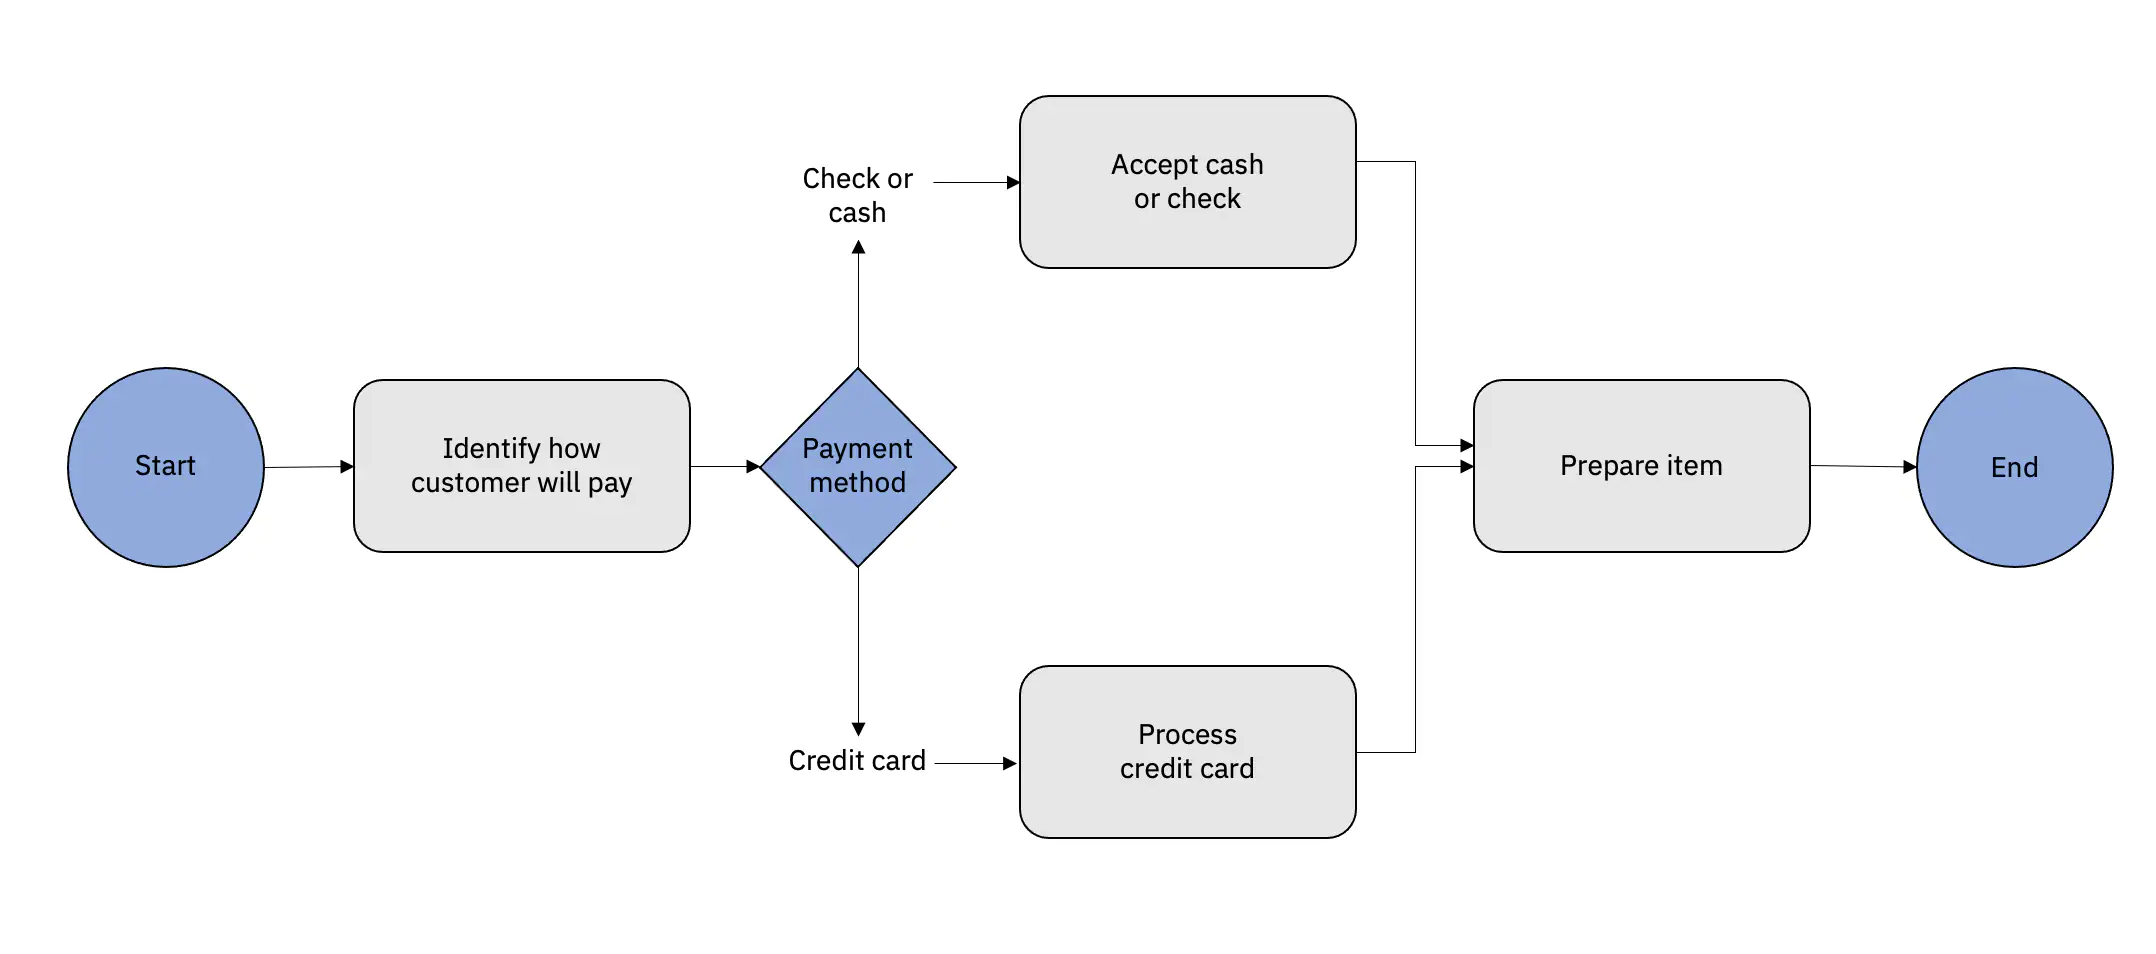
\includegraphics[width=0.7\textwidth]{imgs/BPM/bpmn_diagram.png}
    \caption{Exemplo de um diagrama projetado utilizando BPMN. Imagem da IBM \cite{TheIBM}}
    \label{fig:bpmn_diagram}
\end{figure}

Um conjunto de atividades formam um workflow modelado dentro do software. Esse conjunto de atividades deve ser executado uma ou mais vezes, definindo ações que podem ser executadas para executar um processo. Neste caso, necessitamos que estas atividades estejam separadas para cara execução, para que o dados possam ser registrados para apenas aquela execução.

Para isso, o Flux utiliza de instâncias, que nada mais é que uma separação entre as diferentes execuções de um workflow. Cada instância é criada quando executamos a primeira atividade do workflow selecionado, definindo o início de um novo processo a ser executado.

Um workflow pode ter uma ou mais instâncias, sendo a execução delas o ponto principal do Flux.
Cada workflow pode ser criado através do editor de workflows que existe dentro do próprio Flux, onde podem ser construídos e editados para seguirem um BPM modelado para a organização que irá utilizá-lo.

O editor de workflows funciona de maneira intuitiva para o usuário, sem a necessidade de utilizar nenhuma linguagem de programação, apenas arrastar atributos para atividades criadas e criar atividades seguindo um modelo construído.

Atividades podem ser filhas de outra atividade, ou seja, elas dependem da execução da atividade pai para que elas possam ser executadas, ou podem ser irmãs de outras atividades, que significa que a sua execução não interfere na execução da atividade irmã, mas que as duas só ficam disponíveis quando a atividade pai delas for executada. Podemos visualizar exemplos de workflow na figura \ref{fig:estrutura_workflow}.

\begin{figure}
    \centering
    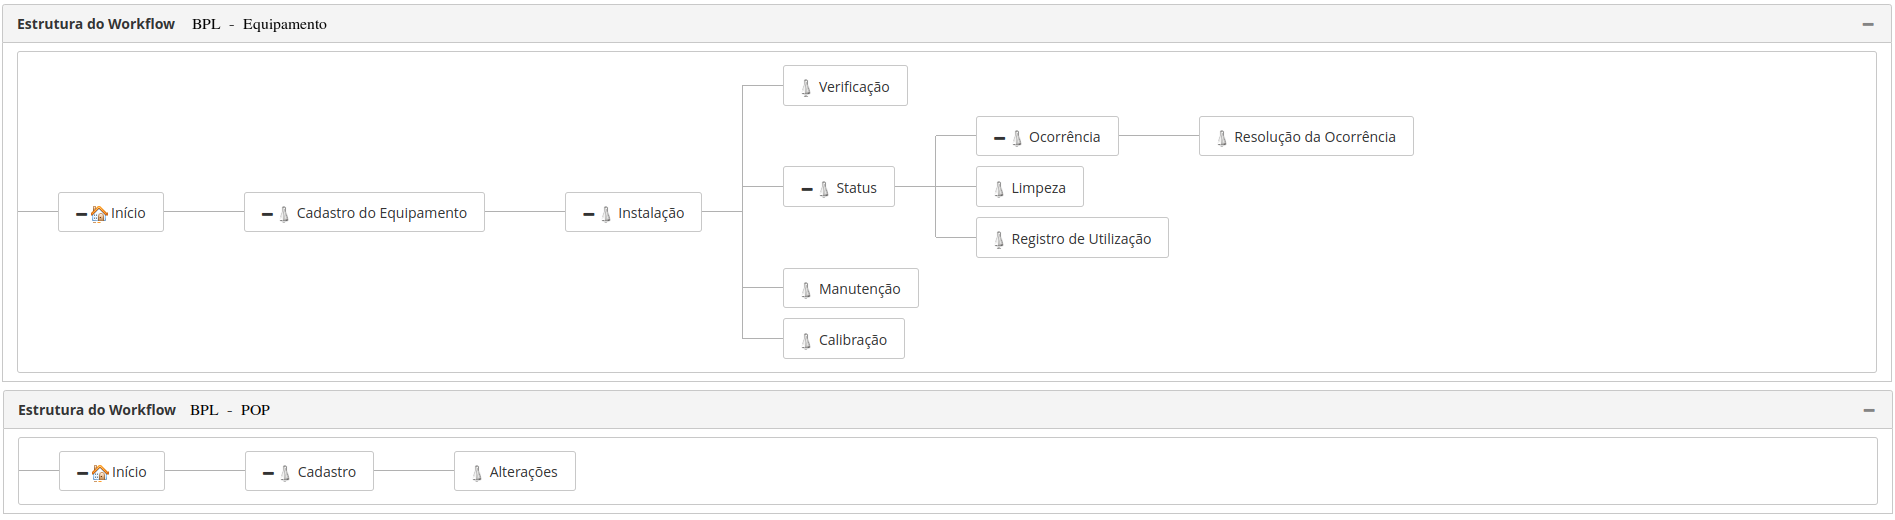
\includegraphics[width=1\textwidth]{imgs/BPL/estrutura.png}
    \caption{Estrutura de dois workflows: BPL - POP e BPL Equipamentos. A atividade inicial destes workflows são as atividades "Cadastro" e "Cadastro do equipamento", respectivamente.}
    \label{fig:estrutura_workflow}
\end{figure}

\subsubsection{Usuários do Flux}

Existem dois tipos de usuários dentro do Flux: Usuários administradores e usuários comuns.

Usuários administradores podem gerenciar todos os quesitos do LIMS para que ele seja moldado para a organização a que pertence. Administradores podem criar workflows dentro do software, configurar permissões de usuários comuns sobre o acesso deles a atividades, instâncias e workflows, além de gerenciar as contas dos próprios usuários comuns.

Os usuários comuns são pessoas que apenas executarão os workflows criados pelos administradores. O usuário comum só poderá visualizar, aprovar, executar, gerar relatórios de atividades que lhe foi dado permissão pelos administradores.

Múltiplos usuários podem executar instâncias diferentes ou até mesmo a mesma instância de um workflow utilizando o Flux. Desta maneira, pode-se integrar múltiplos participantes de um mesmo processo para executarem em paralelo atividades que façam parte do mesmo BPM.